%\makeatletter
%\def\toclevel@chapter{-1}
%\makeatother

\chapter{Conclusion et perspectives}
%\addtocontents{toc}{\bigskip}
%\addcontentsline{toc}{chapter}{Conclusion et perspectives}

Conclusion générique sur les travaux et résultats présentés dans le manuscrit.

travaux sur le temps de diffusion élastique, comparaison avec les fonctions spectrales. Conclusion des deux études: faire attention avec l'utilisation d'approches perturbatives pour un désordre speckle: ça dévie rapidement. la bonne manière d'étudier le temps de diffusion élastique repose sur les fonctions spectrales, c'est à dire la distribution d'énergie de l'état initial dans le désordre.


Expérimentalement, identification et travaux sur les deux limitations identifiées pour la mesure du seuil de mobilité. Nos travaux autour de la chambre de science ont permit d'obtenir de meilleurs condensats, avec un meilleur contrôle des champs magnétiques. Ces travaux ont ainsi permit de récemment obtenir une résolution en énergie de \SI{5}{\hertz}. 




\section{Vers l'étude du régime critique}
ouverture sur la mesure du régime critique, mesures de fonctions spectrales à vitesse non nulle avec un transfert raman. 
\citep{delande2014mobility}
\citep{pasek2017anderson}

\begin{figure}
\centering
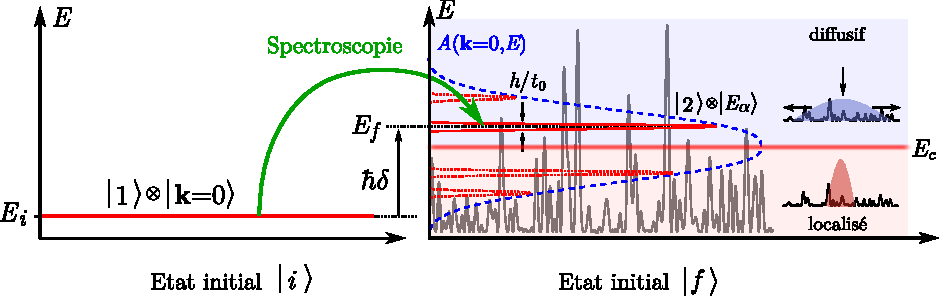
\includegraphics[width=\textwidth]{Fig/Conclusion/spectro_transition_anderson.pdf}
\caption{\textbf{Étude spectroscopique de la transition d'Anderson.} Stuff.}
\label{fig:spectro_transition_anderson}
\end{figure}


\section{Signatures dans l'espace des impulsions}
évolution temporelle de la largeur du pic CBS, contraste du pic CFS qui pourrait être utilisé comme paramètre d'ordre. 

\subsection{Rétro-diffusion cohérente}
\subsection{Diffusion cohérente vers l'avant}

\section{Générer un désordre sur mesure} 
localization landscape, DMD pour autres types de désordre et classes d'universalité...

\section{Autres perspectives}
Effets topologiques sur le graphène qui font de l'anti-localisation: CBS négatif. 

\subsection{Localisation d'Anderson et interactions}
Effet des interactions: many-body localization, verre de bose...
\citep{schreiber2015observation} \citep{choi2016exploring}
\begin{figure}
\centering
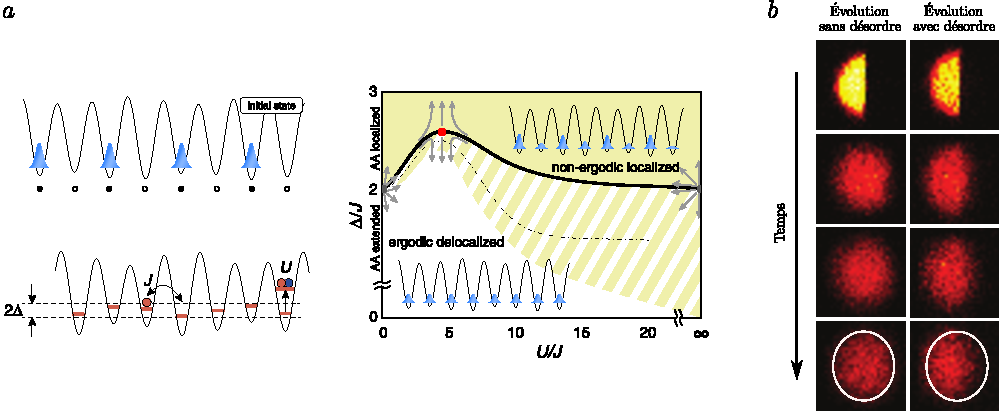
\includegraphics[width=\textwidth]{Fig/Conclusion/many_body_localisation.pdf}
\caption{\textbf{Localisation à $N$-corps.} Stuff. \\
\textbf{corriger figure de gauche.}}
\label{fig:many_body_localisation}
\end{figure}


%\makeatletter
%\def\toclevel@chapter{0}
%\makeatother